\documentclass[12pt]{report}
\usepackage{amssymb,amsmath,latexsym}
\usepackage[framed,numbered,autolinebreaks,useliterate]{mcode}
\usepackage{graphicx}
\usepackage{subcaption}
\usepackage[export]{adjustbox}
\usepackage[square,sort,comma,numbers]{natbib}
\usepackage{algorithm}
\usepackage{algpseudocode}% http://ctan.org/pkg/algorithmicx
% Page length commands go here in the preamble
\setlength{\oddsidemargin}{-0.25in} % Left margin of 1 in + 0 in = 1 in
\setlength{\textwidth}{7in}   % Right margin of 8.5 in - 1 in - 6.5 in = 1 in
\setlength{\topmargin}{-.75in}  % Top margin of 2 in -0.75 in = 1 in
\setlength{\textheight}{9.2in}  % Lower margin of 11 in - 9 in - 1 in = 1 in

\newtheorem{theorem}{Theorem}
\newtheorem{definition}{Definition}

\renewcommand{\baselinestretch}{1.5} % 1.5 denotes double spacing. Changing it will change the spacing
\setlength{\parindent}{0in} 
\begin{document}
\title{Bayesian Statistics and Decision Theory (STAT 565) Final Project:
\\
 Bayesian Inference of Ocean Topography via Internal Waves}
\author{Anil A. Aksu}
\date{\today}
\maketitle
\abstract{In the stratified ocean, the physical processes associated with the turbulence is affected by the bouyancy forces caused by the density gradient in the ocean. Particularly, the wake caused by the underwater vehicle may leave a coherent signal which was transferred by internal Waves to the ocean surface\cite{ThorpeBook}. It carries an information about the turbulent wake to the sea surface which can be detected by means of remote sensing. Similarly, the internal wave field interacting with the topography carries an information about the topography to the sea surface\cite{SutherlandBook}. However, in both cases, these informations obtained are not deterministic, therefore statistical treatment is required. In the analysis presented here, the particular attention is paid to the detection of topography using internal wave field which has important naval engineering applications by means of Bayesian analysis\cite{Hoff}. Finally, the aim of the project is to  .}
\tableofcontents
\listoffigures
\newpage
\chapter{Introduction}

\section{Stratified Ocean}
        
      The ocean is stratified  with an increasing depth. Differential heating is one of the cause leading to that stratification. Sea surface gets exposed to radiative heating more. That causes the stratification in the ocean. The region just below the sea surface is, however, often of almost uniform density to a depth of typically 50 m, but with diurnal, seasonal and latitudinal variations in both density and depth\cite{ThorpeBook}. Below the surface mixed layer, the density increases with depth in a layer known as the pycnocline. Resulting from both gravity and the density stratification, so-called internal waves are generated.But, In  shallow shelf seas, the turbulence caused by the tidal flow over the seabed may dominate, mixing the entire water column, including that near the surface, to a nearly uniform density\cite{ThorpeBook}.
      \begin{figure}[h!]
  \centering
    
    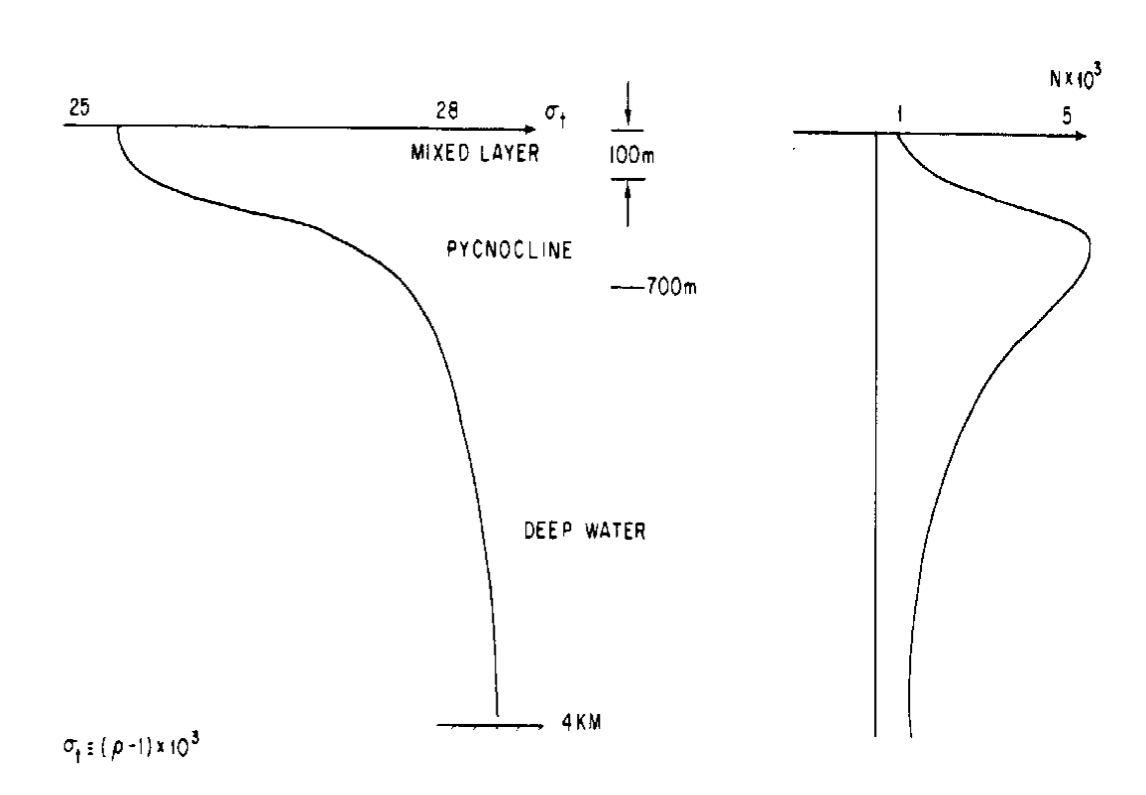
\includegraphics[scale=0.4]{OceanPro.png}   
  \caption{Sample Ocean Density Profile}
           
\end{figure}
When the fluid density is continuously stratified, the oscillatory motion can occur due to differences in buoyancy \cite{LightHillBook} with a frequency $\omega$. These type of waves are commonly called internal gravity waves. In contrast to surface waves, internal waves are not restricted to the interface; they can also propagate vertically \cite{SutherlandBook,LightHillBook}. In the absence of background flow, the dispersion relation of linear internal plane waves can be given as:
 \begin{equation}
 \label{eq:0}
 \omega^2=\frac{N^2 k_{x}^2}{k_{x}^2+k_{z}^2}
\end{equation} 
where $k_x$, $k_z$ are the wavenumbers in $x$ and $z$ directions and $N=\sqrt{(-g/\rho_0)(\mathrm{d}\bar{\rho}/\mathrm{d}z)}$ is the buoyancy frequency, $\mathrm{d}\bar{\rho}/\mathrm{d}z$ is the vertical density gradient, $\rho_0$ is the characteristic density of the stratified fluid. This relation determines both the angle of propagation of an internal wave beam and the direction of the wave number vector. Furthermore, there are several ways that internal gravity waves are generated. The internal waves can be generated by flow over topography. Initially barotropic tidal currents result in baroclinic motion when it interacts with the topography. During the conversion of the energy from barotropic to the baroclinic currents, internal wave beams radiate from the topography\cite{SutherlandBook,LightHillBook}. In general, the internal waves produced do not have a particular forcing frequency but a spectrum of frequencies\cite{ThorpeBook}. $10\%$ of the total energy of the currents is transferred to the internal waves \cite{Kunze}.

 The topographic generation mechanism should be introduced into the numerical model used to study the evolution of an internal wave beam. Recently, considerable attention is paid to understanding generation mechanisms of internal waves numerically \cite{Delwiche,Z&D2013} and experimentally\cite{Allshouse}. Using the results of the analysis and the experiments, a recent theoretical approach by \citet{Aksu2017} derived a governing equation for the time-averaged internal wave propagation. This propagation equation can be used to get theoretical results for the induced internal wave field by the topography. The importance of understanding generation mechanism of internal waves through the interaction with topography has various naval engineering applications such as detection of hidden submarines and continental shelves. Both of these applications also require an approach that first generates a known internal wave field interacting with topography, then measures the perturbation of the internal wave field as shown in figure 1.2. In this way, the theoretical approach\cite{Aksu2017} can be extended to such a problem.

However, by definition of the situation, the possible analysis here is an inverse problem.  Though the physics of the problem guides us to get an insight of the topography. The realization of a practically useful means for predicting the actual geometry of topography is formidable. It is virtually impossible to rationally guess the precise height and the width of the bump in the ocean.  The problem is even more challenging if this identification is to be made in the real application. Here a sample error function is located in a rectangular topography. The motivation of the present study is to solve the inverse problem described above using a Bayesian estimation approach\cite{Reed2015,Lin2017} to identify and characterize the parameters of a simple error function bump where the geometry model is assumed to be perfectly known. 

A common task in this type statistical analysis is to estimate the unknown model parameters associated with the geometry. In the Bayesian approach, the solution covers various possible parameter values\cite{Hoff,Gilks}. Therefore, the Bayesian approach is appropriate for modelling uncertainty in the model parameters. The Bayesian approach is based on prior and likelihood distributions of parameters. The prior distribution includes our beliefs about the problem beforehand, whereas the likelihood represents the probabilities of observing a certain set of parameter values\cite{Hoff,Gilks}. The prior and the likelihood are updated to a posterior distribution, which represents the actual parameter distribution conditioned on the observed data, through the Bayesian rule:
\begin{equation}
\label{eq:1}
f(Z\mid Y)=\frac{f(Z)f(Y\mid Z)}{f(Y)}.
\end{equation}
where the denominator is now expressed as an integral:
\begin{equation}
\label{eq:2}
f(Y)=\int f(Z)f(Y\mid Z)\mathrm{d}Z.
\end{equation}
where $Z,Y$ are continuous random variables. In most cases, this often requires the calculation of complex integrals such as the integral \ref{eq:2}. This integral is often hard to calculate analytically. This problem can be tackled, for example, with Monte Carlo integration methods\cite{Hoff,Gilks} or with Markov Chain Monte Carlo methods\cite{Hoff,Gilks} in which the need for computing these difficult integrals vanishes. 
\\
\\
Furthermore, similar geometric problems are solved using Bayesian analysis by \citet{Lin2017,Reed2015,Earls2013}. Their goal was to determine the presence of structural damage by statistically correlating features extracted from sensor data with data features of known damage. However, this typically requires some a priori knowledge of how the structure will behave when it is damaged. Their solution is to quantify these damage parameters in the finite
element model, so that the model generated response data matches the observed sensor response data. They employed Markov chain Monte Carlo approach\cite{Gilks,Lin2017,Reed2015,Earls2013,Hoff} to successfully characterize the damage, as well as the uncertainty surrounding the parameter estimates.

\newpage
\section{Problem Description And Objectives}

The analysis is numerical and involves the solution of stochastic inverse problem, in a Bayesian setting, in order to quantify uncertainty in modeling parameter estimation describing the topography which can be given as:
\begin{equation}
h(x)=A \int_{-\infty}^{x} e^{-\frac{(x'-x_0)^2}{2\sigma^2}} \mathrm{d}x'
\end{equation}
where $A$ is the characteristic height, $\sigma$ is half-width and $x_0$ is the location of the bump.
\begin{figure}[!h]
 \label{fig:1}
  \centering
      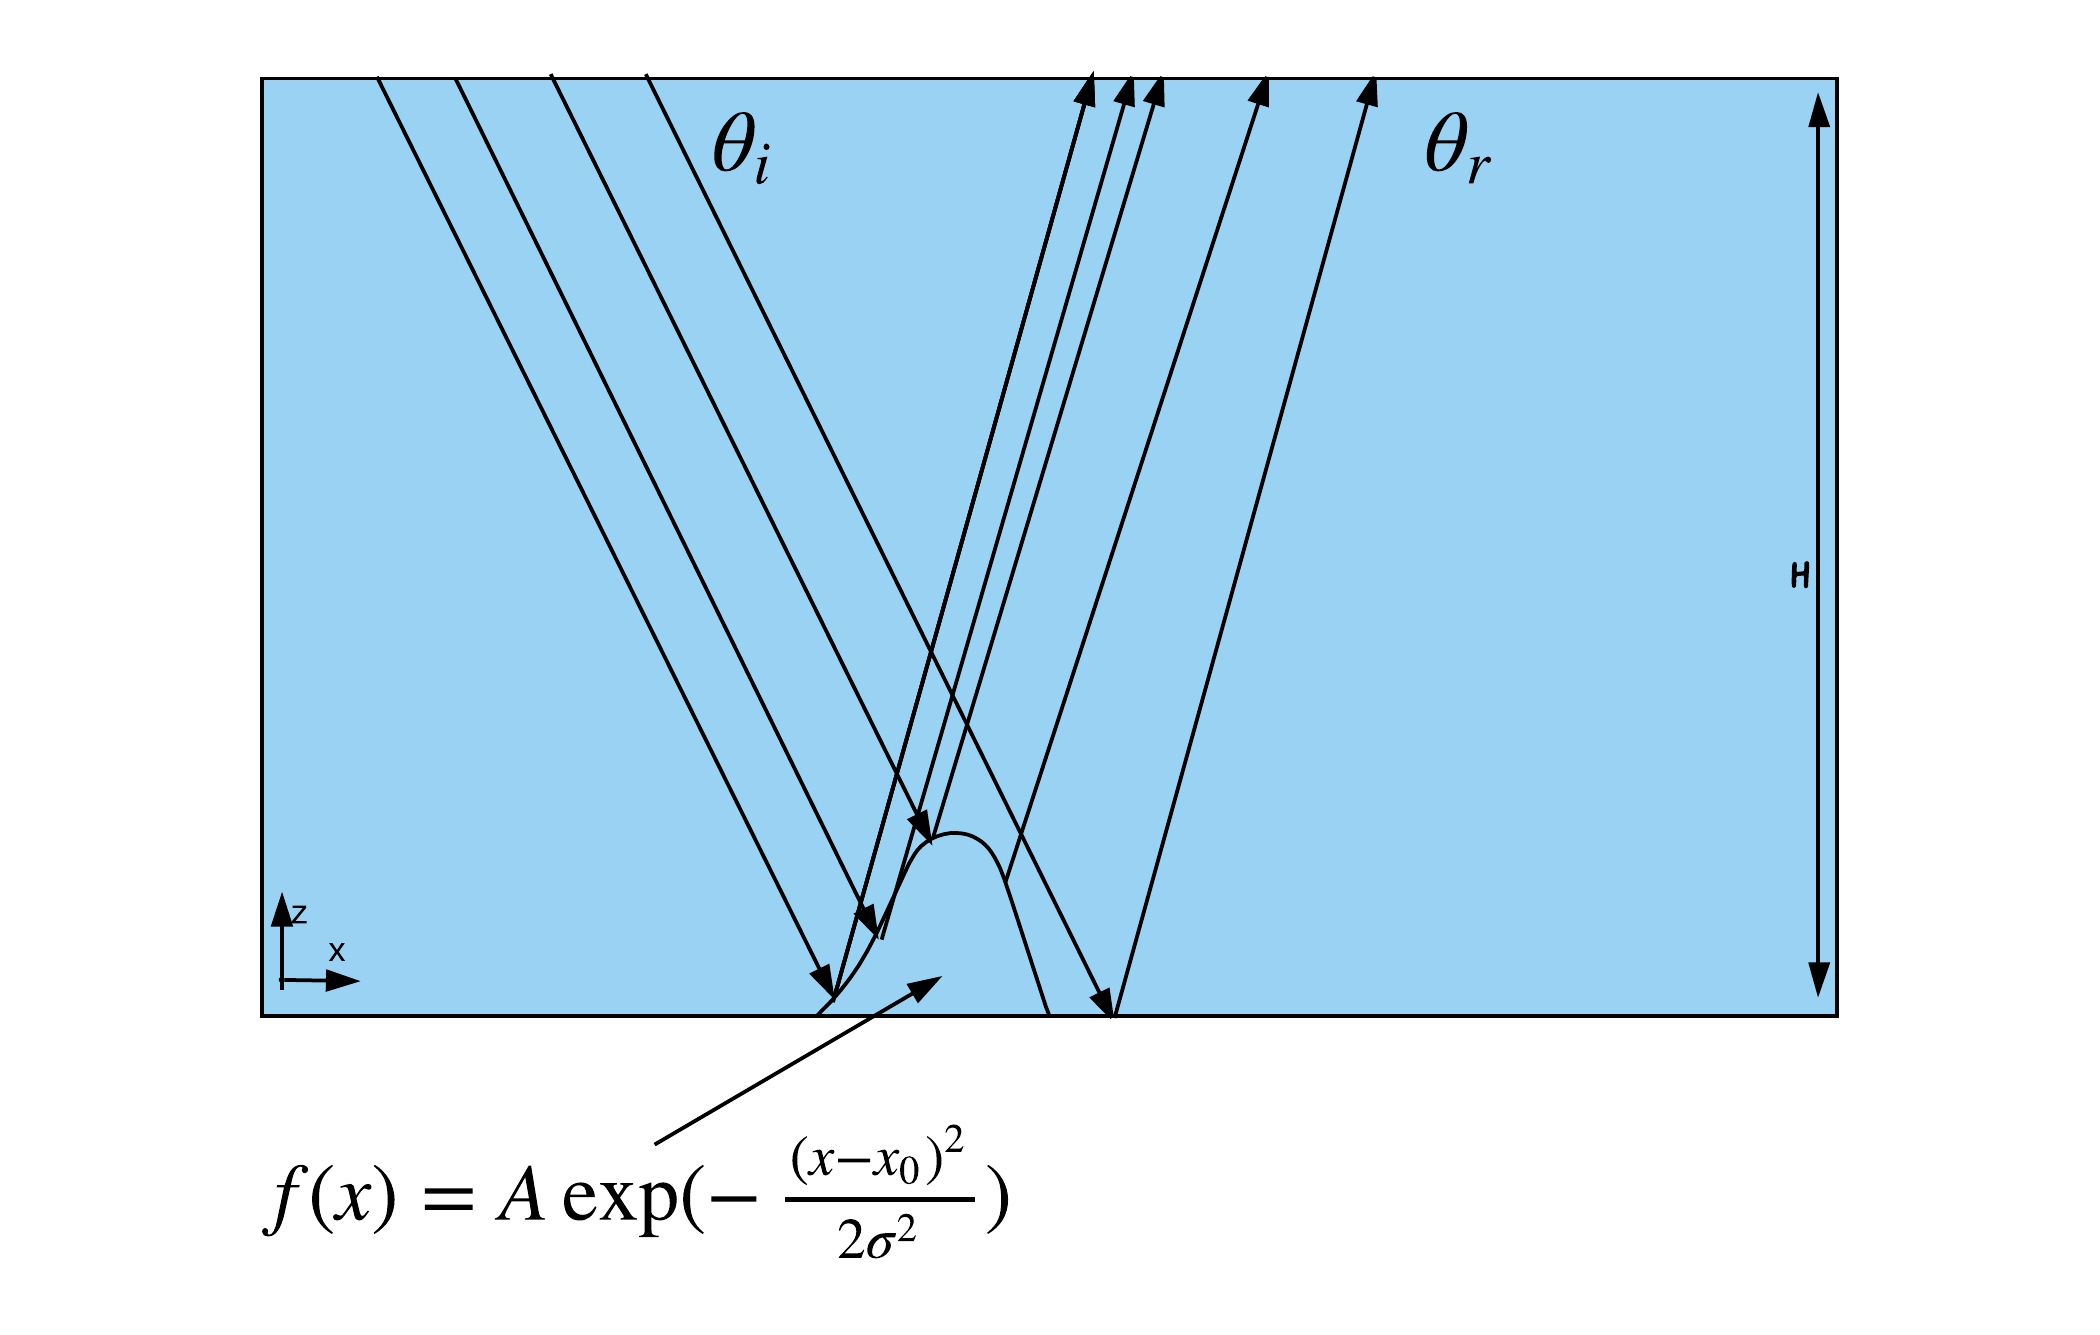
\includegraphics[scale=0.2]{TopoDetect.png}
      \caption{Internal wave field interacting with Gaussian topography.}
\end{figure}
In the real application, an internal wave field is generated by a forcing pedal\cite{Allshouse}, and the perturbation in the field is assumed to be caused by the topography. The data is collected by a sensor nearby the generation location. In addition to the model parameters, there is also an uncertainty associated with measurements of sensors which is introduced as a white noise similar to the previous studies\cite{Lin2017,Earls2013,Reed2015}. The full physical model described in the chapter \ref{chap:analysis} is a non-linear model, however it can be linearized by taking natural logarithm of both sides of the full physical model. After defining the physical model, white noise is introduced. Metropolis-Hastling algorithm\cite{Solonen2006} is used to obtain the posterior distribution of the coefficients of linear Bayesian fit and the white noise. Finally, The objectives of the analysis presented here can be summarized as: 
\begin{itemize}
   \item Derive a physical model which describes the perturbation of the internal wave field due to an irregularity (bump) on the topography
   \item  Derive a statistical model which includes the geometric parameter associated with the topography.
   \item  Obtain the posterior distribution of the determined geometric parameters.
   \end{itemize}
   
\chapter{\label{chap:analysis} Analysis}

\section{Internal wave beam reflection from a surface with a bump }
The internal wave beams generated by the interaction between a tidal current with topography as explained by \citet{Kunze} can be in various forms. In some numerical simulations, this generation mechanism can be replaced with a virtual forcing pedal as shown by \citet{Delwiche,Z&D2013} to generate an internal wave beam with a specified wave number and frequency. The total energy is given by \citet{Aksu2017} as:
\begin{equation}
\label{eq:12}
<E>=<E_k>+<E_p>=\epsilon^2\frac{\rho_0}{2}(\vec{A}_{inc}\cdot\vec{A}_{inc}).
\end{equation}
 The steady-state response of the energy equation\cite{Aksu2017} is given as:
\begin{equation}
\label{eq:20}
\mathbf{\nabla}\cdot(\vec{Cg}<E>)=-\frac{\nu N^2k_{x}^2}{\omega^2}<E>+\gamma A_{inc}^{x}F.
\end{equation}
where $\vec{Cg}=\partial \omega / \partial k_x \vec{i},\partial \omega / \partial k_z \vec{k}$ and the viscous dissipation term $\nu N^2k_{x}^2/\omega^2$. In case of a linear stratification, the group velocity is constant along the intern wave beam path, this will enable us to simplify the equation \ref{eq:20}. The new coordinate system $\xi-\eta$ is introduced. $\eta$ is in the direction of the wave number vector $\vec{k}$ and $\xi$ in the direction of the group velocity vector $\vec{Cg}$.The resultant integral gives us the distribution of the velocity amplitude along the propagation direction. Moreover this integral converges to certain value after $\xi > 2\sqrt{2} \sigma+\alpha\sigma^2 $ which can be given as:
\begin{equation}
\begin{split}
A_{inc}^{x}=A_0 \exp(-\alpha\xi)\exp(-\frac{\eta^2}{2\sigma^2}).
\end{split}
\end{equation}
Moreover, virtual forcing is negligible in the reflection region. Therefore, the governing equation for the reflecting internal wave beam can be written as:
\begin{equation}
\label{eq:40}
\mathbf{\nabla}\cdot(\vec{Cg}_{ref}<E_{ref}>)=-\frac{\nu N^2k_{x}^2}{\omega^2}<E_{ref}>.
\end{equation}

The magnitude of the reflecting group velocity vector $\vec{Cg}_{ref}$ is the same as the incident group velocity vector $\vec{Cg}$. However it propagates downwards, therefore, explicitly the reflecting group velocity vector can be given as $Cg_{ref}^x=Cg^x$ and $Cg_{ref}^z=-Cg^z$. Similar to the incident internal wave beam, a new coordinate system $\xi_r-\eta_r$ is introduced. Note that $r$ subscript stands for denoting reflection. Again, $\eta_r$ is in the direction of the wave number vector $\vec{k}$ and $\xi_r$ in the direction of the group velocity vector $\vec{Cg}_{ref}$. Explicitly, the relation between $x-z$ coordinate system and $\xi_r-\eta_r$ coordinate system can be given as:
\begin{equation}
\begin{bmatrix}
\xi_r\\ 
\eta_r
\end{bmatrix}
=
\begin{bmatrix}
\cos \theta_r & \sin \theta_r \\ 
 -\sin \theta_r & \cos \theta_r 
\end{bmatrix}
\begin{bmatrix}
x\\
z 
\end{bmatrix}
\end{equation}
where $\theta_r=\tan^{-1}(-k_x/k_z)$.
In this configuration, it is assumed that there is no displacement on boundaries, therefore the displacement field can be given as:
\begin{equation}
\label{eq:20}
\vec{u}\cdot \vec{n}=0.
\end{equation}
where $\vec{u}_0 + \epsilon \vec{u}_1$ and also the unit vector $\vec{n}$ is defined as:
\begin{equation}
\vec{n}=\mathbf{\nabla}\Omega.
\end{equation}
where $\Omega(x,y)=y-A\int_{-\infty}^x e^{-\frac{(x'-x_0)^2}{2\sigma^2}}\mathrm{d}x'$. Note that $A<<1$ therefore it is assumed that the anomaly height is small compared to the domain height $H$. As a result, the unit vector can be given as:
\begin{equation}
\vec{n}=\hat{y}+A e^{-\frac{(x-x_0)^2}{2\sigma^2}}\hat{x}.
\end{equation}
Therefore the condition \ref{eq:20} results in the following conditions as powers of $A$. At the leading order $O(1)$:
\begin{equation}
u_{y}^{0}=0,
\end{equation}
At the order $O(A)$:
\begin{equation}
u_{y}^{1}+u_{x}^{0}A e^{-\frac{(x-x_0)^2}{2\sigma^2}}=0.
\end{equation}

\section{Bayesian Analysis}

In the case of the interaction between the topography and the internal wave field also a sensor noise will contribute the model which can be given as:
\begin{equation}
\label{eq:21}
\log(u_{y}^{1})=-\log(u_{x}^{0})+\log(A)-(2\sigma^2)^{-1} (x-x_0)^2.
\end{equation}
The physical model described in equation\ref{eq:21} can be re-formulated as:
\begin{equation}
u_{i}^{1}=f_i(\mathbf{\theta})+\eta_i
\end{equation}
where $\mathbf{\theta}=(\sigma^2,A)$ and $\eta_i$ are independent and identically distributed
(i.i.d.) errors taken from a zero-mean, Gaussian distribution with variance $\sigma_{\eta}$ by \citet{Reed2015}. Given this assumed noise distribution, the probability of observing the value $u_{i}^{1}$ can be modelled as:
\begin{equation}
\label{eq:22}
f_{\eta}(u_{i}^{1}\mid f_i(\mathbf{\theta}))=\frac{1}{\sqrt{2\pi \sigma_{\eta}}}e^{-\frac{1}{2 \sigma_{\eta}^2}((u_{i}^{1}-f_i(\mathbf{\theta}))^2}.
\end{equation}
Equation \ref{eq:22} includes the effects of uncertainty due to measurement and noise. As a result, we formed multivariate analysis model for the physical problem. The formulation used here is also similar to the formulation used by \citet{Lin2017,Earls2013,Reed2015}. 
\subsection{Metropolis Algorithm}
The Metropolis-Hastings (MH) algorithm simulates samples from a probability distribution by making use of the full joint density function and proposal distributions.
\begin{algorithm}
\caption{Metropolis Hastling Algorithm}\label{MetroHastle}
\begin{algorithmic}[1]
\Procedure{Metropolis Hastling Algorithm}{}
\State $\textit{Initialize $\theta_0 \sim q(\theta)$}$
\For{iteration $k=1,2,...,n$} 
\State $\textit{Propose: $\theta^* \sim q(\theta^{k} \mid \theta^{k-1})$}$
\State $\textit{Acceptance probability:}$
\State $\textit{$\alpha(\theta^*,\theta^k)= \min\left \{ 1, \frac{p(\theta^*)q(\theta^k \mid \theta^k)}{p(\theta^k)q(\theta^* \mid \theta^k)}  \right \}$}$
\State $\textit{$u \sim Uniform(0,1)$}$
\If{$u< \alpha$}
\State $\textit{Accept the proposal: $ \theta^{k} \leftarrow \theta^*$}$
  \Else
\State $\textit{Reject the proposal: $ \theta^{k} \leftarrow \theta^{k-1}$}$
  \EndIf
\EndFor

\EndProcedure
\end{algorithmic}
\end{algorithm}

 The MH algorithm starts with generating a candidate sample $\theta_{1}$ from the proposal distribution $q(·)$. These candidate samples are accepted probabilistically based on the acceptance probability $α(·)$ defined as:
\begin{equation}
\alpha(\theta^*,\theta^k)= \min\left \{ 1, \frac{p(\theta^*)q(\theta^k \mid \theta^k)}{p(\theta^k)q(\theta^* \mid \theta^k)}  \right \}.
\end{equation} 
where $k$-th iteration we have $(\theta^1,\theta^2,...,\theta^k)$. The $(k+1)$st iteration first generates $\theta^*$ from a proposal density $q(\theta^* \mid \theta^k)$. This density should converge to the actual posterior distribution in theory. There are mainly two kinds of proposal distributions, symmetric and asymmetric. A proposal distribution is a symmetric distribution if $q(\theta^k\mid \theta^{k−1})= q(\theta^{k−1}\mid \theta^k)$. Straightforward choices of symmetric proposals include Gaussian distributions centered at the current state of the chain which is the choice used in the problem here. For example, if we have a Gaussian proposal, then we have $\theta^* = \theta^{k-1}+\mathcal{N}(0; \sigma)$. Because the pdf for $\mathcal{N}(\theta^*-\theta^{k-1}; 0; \sigma) = \mathcal{N}(\theta^{k-1}-\theta^*; 0; \sigma)$, this is a symmetric proposal. This proposal distribution randomly perturbs the current state of the chain, and then either accepts or rejects the perturbed value. 
 
Intuitively, the MH acceptance function is designed to keep a balance between the following two constraints. First, The sampler should tend to visit higher probability areas under the full joint density. Secondly, the sampler should explore the space and avoid getting stuck at one site. The sampler can reverse its previous move in the space; this constraint is given by the ratio $\alpha$. It is important that the MH acceptance function has this particular form because this form
ensures that the MH algorithm satisfies the condition of detailed balance, which guarantees
that the stationary distribution of the MH algorithm is in fact the target posterior that we
are interested in.

Finally, we accept a given proposal with the acceptance probability $\alpha$ which is the outcome of the acceptance function described above. The $min$ operator in the acceptance function makes sure that the acceptance probability $\alpha$ is never larger than 1. Operationally, we draw a random number from uniform distribution centred around $\theta^{k-1}$, and if this value is smaller than $\alpha$, we accept the proposal; otherwise we reject it. Thus
\begin{equation}
\theta^{k+1}= 
\left\{\begin{matrix}
\theta^* & \text{with probability} & \alpha(\theta^*,\theta^k)\\ 
\theta^{k} & \text{with probability} & 1- \alpha(\theta^*,\theta^k) 
\end{matrix}\right.
\end{equation}

\newpage 




\chapter{Results}
This part discusses results obtained using the Bayesian approach for the topography detection. In this cases, results from the Metropolis-Hastling exploration of the Bayesian posterior, describing the geometry of the topography, is presented. 
\begin{figure}[!h]
 \label{fig:Posterior}
  \centering
      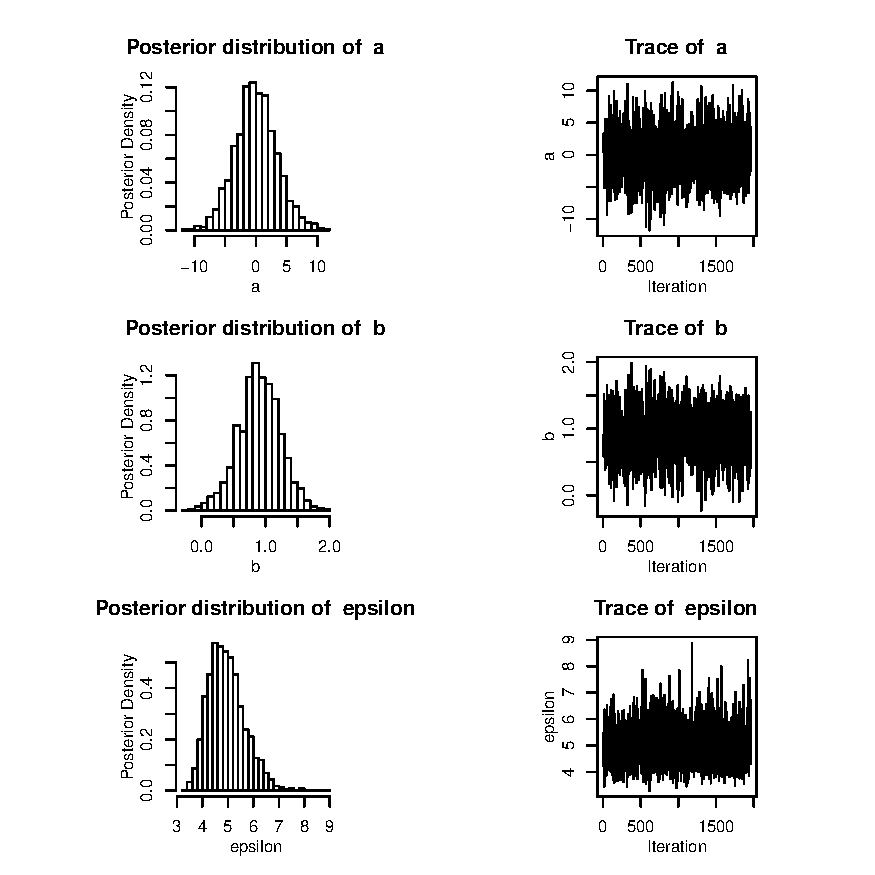
\includegraphics[scale=0.6]{PosteriorDistribution}
      \caption{Posterior Distributions.}
\end{figure}

The linear model proposed in chapter \ref{chap:analysis} can be given as:
\begin{equation}
y_i=a+bx_{i}^2+\eta_i
\end{equation}
where $a=\log(A)$, $b=(2\sigma^2)^{-1}$. These results are the foundation of the more complex analysis conditions. In the analysis presented here, the geometry of the topography is prescribed, however similar type of analysis can be extended to unknown topographies.

 
\chapter{Conclusion}
In this analysis, both the modeling and estimation tools needed to successfully identify and characterize the topography are described. A Bayesian approach to topography parameter estimation is adopted, whereby the unknown parameters describing the topography are treated as random variables; each described by a probability density function. It is shown how numerical samples from these functions can be obtained and subsequently used to estimate the error associated with the topography parameters, independent of $\sigma_{\eta}$. The Bayesian analysis in the current approaches provides both parameter estimates and quantify the uncertainty in the predictions of the parameters.
\appendix


\chapter{\label{app:1} R Codes}

\lstinputlisting[caption={R Code of Metropolis Hastling Algorithm for Topography Detection via Internal Wave Field}]{MetroHastle.R}
\lstinputlisting[caption={R Code for Internal Wave Field Perturbation}]{getPerturbWave.R}


\bibliographystyle{plainnat}
\bibliography{Bayes}% Produces the bibliography via BibTeX.

\end{document}
